\chapter{datareset} \label{datareset}

\section{Introduction}

The \texttt{datareset} command assumes that certain parameters of the LPE determine which summands can be followed by which summands.
These parameters determine the control-flow of the LPE, and are therefore called \emph{control-flow parameters}.

\emph{Data parameters}, on the other hand, are used to store values, and often temporarily, which means that their values may not be used anymore after a particular state.
Data parameters can typically have different values after such a state, which causes them to add states to the state space for each of those values -- \emph{without} adding any new behavior!

The \texttt{datareset} command attempts to detect LPE control-flows and determine the parts of those control-flows where data parameters are no longer used.
At these locations, data parameters are set to a default value (`reset').
This removes states from the state space, potentially improving performance of subsequent computations.

\section{Formal background}

The control-flow analysis is based on work done in \cite{van2009state}.

\subsection{Parameter properties}

Each parameter $p$ of a summand $s$ has the following properties:
\begin{itemize}

\item Is the value of $p$ potentially altered by $s$?
If so, $p$ receives the label `changed'.

\item Does $p$ occur in the guard of $s$?
If so, $p$ receives the label `directly used'.

\item Has $p$ received the label `directly used' in $s$?
Or does $p$ occur in the assignment by $s$ to a parameter that has received the label as `changed'?
In either case, $p$ also receives the label `used'.

\item Must the value of $p$ have a specific (unique) value $v$ in order for $s$ to be enabled?
If so, $p$ receives the label `having a source' for $s$, with the source being $v$.

\item Does the value of $p$ have a specific (unique) value $v$ immediately after $s$ has been applied?
If so, $p$ receives the label `having a destination' for $s$, with the source being $v$.

\item Does $p$ have both a source and a destination for $s$?
Then $p$ is called a \emph{ruling parameter}, and $p$ is said to `rule' summand $s$.

\end{itemize}

\subsection{Control-flow graphs}

A parameter of the LPE is a \emph{control-flow parameter} of the LPE if for all summands it is either a ruling parameter or not \labeledas{changed} (or both).
A parameter that is not a control-flow parameter is defined as a \emph{data parameter}.

\vspace{1mm}

For each control-flow parameter $f$ of the LPE, a control-flow graph is constructed.
There is a state in the control-flow graph for each source and destination of $f$ (across all summands).
Two states $s_1$ and $s_2$ are connected by an edge $(s_1, i, s_2)$ if there is a summand $i$ where the source of $f$ is represented by one of the states and where the destination of $f$ is represented by the other state.
The direction of such an edge is from source state to destination state.

\subsection{Belongs-to function}

Here, the \emph{belongs-to} function is introduced.
The belongs-to function maps each data parameter $d$ to some set of control-flow parameters $b(d)$ as follows

\begin{align*}
b(d) = F \cap \bigcap\limits_{s \in S}^{} \text{ruling}(s)
\end{align*}

where

\begin{itemize}
\item $F$ is the set of all control-flow parameters;
\item $S$ is the set of all summands in which $d$ is \labeledaseither{changed}{used};
\item $\text{ruling}(s)$ is the set of all parameters that rule summand $s$.
\end{itemize}

\section{Algorithm}

The algorithm executes 3 phases: the preparatory phase, the iterative phase, and the deletion phase.

\subsection{Preparatory phase}

In this phase, the parameter properties, control-flow graphs and belongs-to function are computed.

\subsection{Iterative phase}

In the iterative phase, the so-called \emph{relevance relation} is computed.
This relation, with symbol $R$, relates a data parameter $d$, a control-flow parameter $f$, and a value $v$ if $d$ is `relevant' after a state in which $f$ has value $v$.
This is denoted $R(d, f, v)$.
Intuitively, this is a situation in which $d$ should \emph{not} be reset because its value may be needed in the future.

The computation of $R$ is a fixpoint algorithm: modifications are applied iteratively until $R$ no longer changes.
The initial value of $R$ is set to
\begin{align*}
R_0 = \bigcup\limits_{\substack{i \in S \\ d_k \in \text{directlyUsed}(i)}}^{} \;\{\; (d_k, d_j, \text{source}(i, d_j)) \;|\; d_j \in b(d_k) \;\}
\end{align*}

where

\begin{itemize}
\item $S$ is the set of all summands;
\item $\text{directlyUsed}(i)$ is a function that gives the set of all parameters that are \labeledas{directly used} in a summand $i$;
\item $\text{source}(i, f)$ is a function that gives the source value of a control-flow parameter $f$ for a summand $i$.
\end{itemize}

Each iteration can be split into two steps.
The first step checks for control-flow graphs in which a data parameter $d$ has already been \labeledas{relevant} whether this implies that $d$ is also relevant in preceding states (of the same control-flow graph).
If so, the appropriate triples are added to $R$:
\begin{align*}
R_{n}{'} = R_{n-1} \cup \bigcup\limits_{\substack{i \in S}}^{} \;\left\{\; (d_k, d_j, s) \;\middle|\; \substack{(d_l, d_j, t) \in R_{n-1} \\ d_j \in b(d_k) \\ d_k \in \text{vars}(v_i(d_l)) \\ (s, i, t) \in E_{d_j}} \;\right\}
\end{align*}

where

\begin{itemize}
\item $E_{f}$ is the set of edges that are part of the control-flow graph of control-flow parameter $f$.
\end{itemize}

The second step is similar, but data parameters that are found to be relevant are added as triples to $R$ in relation to \emph{another} control-flow parameter:
\begin{align*}
R_{n} = R_{n}{'} \cup \bigcup\limits_{\substack{i \in S}}^{} \;\left\{\; (d_k, d_j, \text{source}(i, d_j)) \;\middle|\; \substack{(d_l, d_p, t) \in R_{n}{'} \\ d_j \in b(d_k),\; d_j \notin b(d_l) \\ d_k \in \text{vars}(v_i(d_l)) \\ (r, i, t) \in E_{d_p}} \;\right\}
\end{align*}

\subsection{Deletion phase}

Finally, each summand of an LPE is subject to modification.
Modifications are made by making use of the belongs-to function $b$ and the relevance relation $R$.
Intuitively, we check whether the value of a parameter is `relevant' after a specific summand $i$ has been applied.
If so, the parameter should not be reset.
Otherwise, the parameter can be reset, for example to its initialization value:

\begin{align*}
v_{i}{'}(d_k) = \begin{cases}
v_{i}(d_k) & \text{if } \bigwedge\limits_{\substack{d_j \in \text{ruling}(i) \\ d_j \in b(d_k)}}^{} R(d_k, d_j, \text{dest}(i, d_j)) \\
v_{I}(d_k) & \text{otherwise}
\end{cases}
\end{align*}

where

\begin{itemize}
\item $\text{ruling}(s)$ is the set of all parameters that rule summand $s$;
\item $\text{source}(i, f)$ is a function that gives the destination value of a control-flow parameter $f$ for a summand $i$.
\end{itemize}

\section{Benchmark results}

The following durations were measured with a benchmark for several models:
\begin{itemize}
\item The average duration of \txs{} to make 500 steps in a model after it has been converted to LPE form;
\item The average duration of \txs{} to make 500 steps in a model after it has been converted to LPE form and after the \texttt{datareset} operation has been applied.
\end{itemize}

When plotting the second series of measurements against the first (see Figure~\ref{datareset-vs-lpe-only:fig}), it is easy to see that the impact is insignificant in most cases.

\begin{figure}[!ht]
\begin{center}
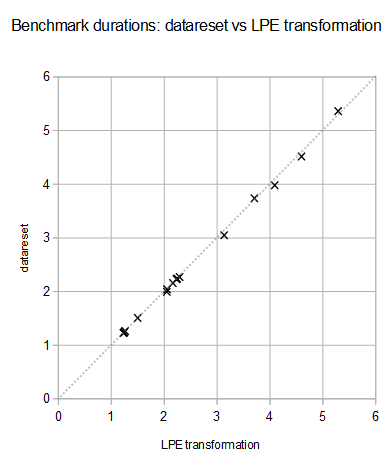
\includegraphics[width=0.7\linewidth]{charts/datareset-vs-lpe-only}
\caption{Benchmark results: datareset vs LPE transformation}
\label{datareset-vs-lpe-only:fig}
\end{center}
\end{figure}

